Les systèmes critiques natifs du cloud dépendent de plus en plus de Kubernetes pour orchestrer et gérer des services interdépendants~\cite{Pahl2019}. HPA est un mécanisme largement adopté pour ajuster dynamiquement le nombre de pods en fonction de l'utilisation des ressources, permettant ainsi aux systèmes de gérer des charges de travail très dynamiques~\cite{Toka2020}. Cependant, des défaillances telles que les plantages de pods, les conflits de ressources et les goulots d'étranglement peuvent gravement compromettre les performances de toutes les fonctionnalités du cluster, que nous appelons globalement « résilience opérationnelle~\cite{burns2016borg}». Pire encore, ces défaillances peuvent être exploitées par des attaquants pour dégrader les performances ou provoquer des pannes, comme on le voit dans des contextes hostiles tels que les attaques DDoS~\cite{David2021}.

Bien que les attaques DDoS puissent sembler improbables dans des clusters d'entreprise isolés, de nombreuses organisations exposent leurs services via des passerelles d'entrée, ce qui en fait des cibles viables. En interne, des surcharges de type DDoS peuvent également résulter de configurations incorrectes, de dispositifs compromis ou d'exercices de red teaming. La prise en compte de tels scénarios adversaires s'inscrit dans les meilleures pratiques en matière de cybersécurité et contribue à garantir une auto-scaling robuste et tolérante aux pannes.

Dans de tels scénarios hostiles, des acteurs malveillants peuvent exploiter les mécanismes de mise à l'échelle, exposant ainsi les limites des systèmes HPA conventionnels. Les approches modernes ont cherché à combler ces lacunes en utilisant l'apprentissage par renforcement (RL), dans lequel un agent optimise un objectif global unique, tel que la minimisation de la latence ou de l'utilisation des ressources~\cite{Gari2021}. Si ces méthodes démontrent leur adaptabilité, elles s'avèrent souvent insuffisantes pour gérer divers scénarios de défaillance afin de maintenir la \textit{qualité de service} (QoS)~\cite{Liu2024}. Par exemple, il peut être beaucoup plus critique de donner la priorité aux réponses aux pannes en cascade des pods lors d'une attaque que de réduire la latence. Ces défis soulignent la nécessité d'un système d'auto-scaling capable d'équilibrer dynamiquement plusieurs sous-objectifs afin de maintenir toute la QoS et de maximiser la résilience opérationnelle.

Passer d'une optimisation à objectif unique à une approche multi-objectifs est complexe~\cite{Shoham2009MAS}. Dans des scénarios réels, la résilience opérationnelle ne peut se réduire à un seul objectif : l'optimisation de la latence peut entrer en conflit avec la garantie d'une haute disponibilité ou la limitation du surprovisionnement des ressources. Dans des conditions difficiles, par exemple, la priorité accordée à l'atténuation des attaques DDoS peut nécessiter de sacrifier la latence, tandis que la récupération après un crash de pod exige une réaffectation rapide des ressources. Un agent RL unique a du mal à répondre à ces priorités en raison de la difficulté à coordonner les réponses à des défaillances diverses~\cite{Jennings1998}.

En revanche, les MAS offrent un paradigme prometteur en décomposant l'objectif global de maximisation de la résilience opérationnelle en sous-objectifs gérés par des agents spécialisés~\cite{Shoham2009MAS}. Chaque agent se concentre sur un mode de défaillance ou un objectif de performance spécifique, ce qui facilite la spécialisation, améliore la coordination et permet un apprentissage évolutif des politiques dans le cadre de charges de travail dynamiques.

Dans un scénario antagoniste, chaque défenseur peut contribuer de manière collaborative à des actions d'échelle complémentaires afin d'atteindre son propre sous-objectif, ce qui permet des réponses plus résilientes et mieux adaptées au contexte face à un attaquant~\cite{Jennings1998}. Nous appelons l'ensemble de ces collaborations un HPA MAS. Un HPA MAS s'appuie en fait sur le cadre de cyberdéfense des agents autonomes intelligents de cybersécurité (AICA), qui peuvent être considérés comme des agents ayant des rôles et des missions spécialisés qui défendent en collaboration les systèmes contre les attaquants~\cite{Kott2018}.

% Problématique
Cependant, la conception de HPA MAS adaptés à un cluster présente des défis importants, tels que la nécessité d'une connaissance approfondie du cluster, la nature fastidieuse des processus de conception manuelle et la difficulté de garantir un comportement optimal des agents. De plus, les changements de cluster nécessitent de répéter le processus de conception, ce qui augmente les coûts opérationnels et la complexité.


\subsection{Description du cluster Kubernetes et de sa configuration}

L'environnement d'évaluation se compose d'un cluster Kubernetes simulant une architecture \textbf{Chained Services} (CS). Chaque service comprend un ensemble de microservices hébergés dans des pods et gérés par des déploiements. Par exemple, \autoref{fig:chained_services_graph} illustre la représentation graphique d'un cluster CS à quatre services. Nous avons envisagé d'utiliser un cluster caractérisé par les spécifications suivantes :

\begin{itemize}
    \item \textbf{Topologie :} Quatre services interconnectés en cours d'exécution, configurés pour émuler des conditions réelles, notamment des conflits de ressources, des goulots d'étranglement et des scénarios adversaires ;
    \item \textbf{Simulation de défaillance :} les goulots d'étranglement et les défaillances en cascade sont induits par des charges de travail gourmandes en ressources, tandis que les conditions adverses (par exemple, les attaques DDoS) sont émulées à l'aide de Locust~\cite{locust2021} et de scripts personnalisés basés sur le hasard ;
    \item \textbf{Nœuds de travail :} 1 nœud de travail avec 8 vCPU, 32 Go de RAM et une bande passante réseau de 1 Gbps. Cette configuration est adaptée à des fins de test sur des clusters de taille moyenne ;
    \item \textbf{Nœud d'entraînement :} 1 cluster à haute puissance de calcul composé de nœuds équipés de GPU NVIDIA Tesla V100 (16 Go), de processeurs Intel Xeon Platinum (2,3 GHz, 16 cœurs) et de 128 Go de RAM.
\end{itemize}

\begin{figure}[h!]
    \centering
    \hspace{-0,4cm}
    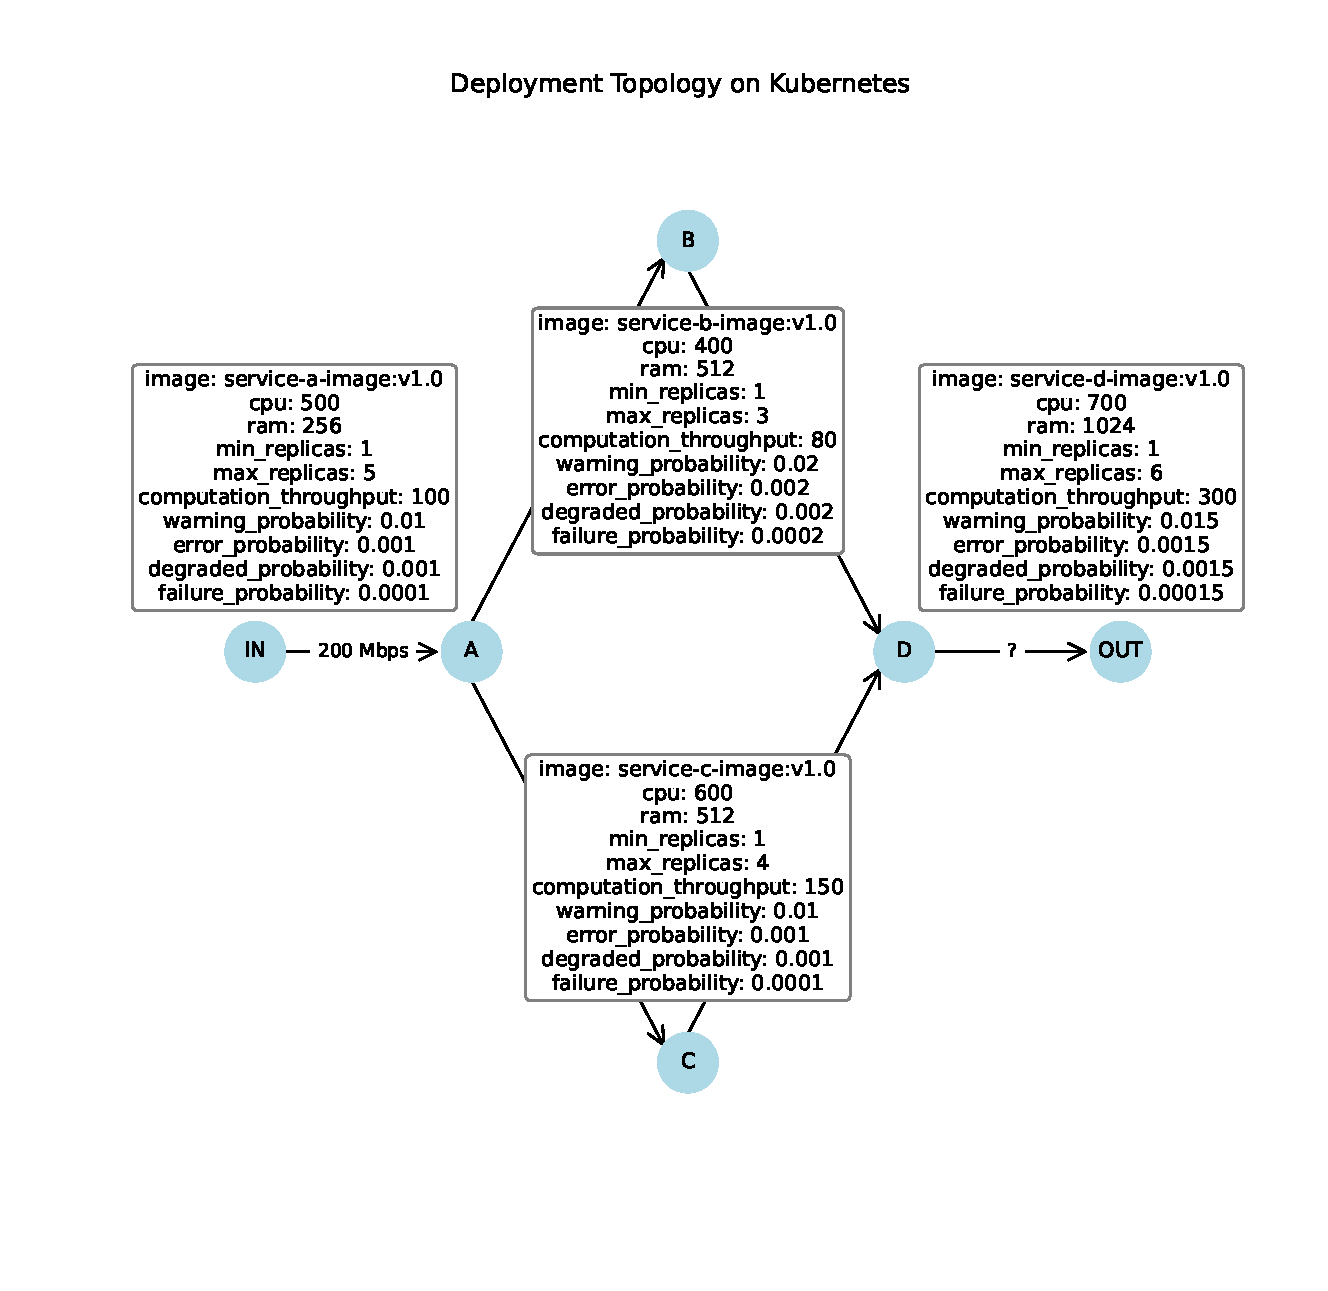
\includegraphics[trim=1.8cm 3.3cm 1.25cm 3.5cm, clip, width=0.5\textwidth]{figures/k8s_cluster_graph.pdf}
    \caption{Représentation graphique d'un cluster « Services en chaîne » avec quatre services}
    \label{fig:chained_services_graph}
\end{figure}

\subsection{Implémentation de KARMA avec CybMASDE}

% À FAIRE :
% - Présenter le framework CybMASDE
% - Scénario normal, scénario DDoS (augmentation ponctuelle du volume de données), scénario de défaillance (corruption ponctuelle des données), scénario de contention de ressources (priorisation), scénario mixte
% - Protocole d'expérimentation
%   - Baseline 1 : Agent unique sans spécifications organisationnelles souples
%   - Référence 2 : agent unique avec spécifications organisationnelles rigides
%   - Référence 3 : multi-agent sans spécifications organisationnelles
%   - Référence 4 : multi-agent avec spécifications organisationnelles

\footnotetext[2]{\label{lnk:footnote_2}Dans notre implémentation par défaut, $\alpha = 3$, $\sigma = 10$, $\kappa = 1$, $ch = 1$, poids des récompenses $(w_1, w_2, w_3, w_4, w_5) = (0,2, 0,2, 0,2, 0,2, 0,2)$, $Q_{\text{seuil}} = 30$ et $U_{\text{seuil}} = 90\%$.
    Le code source de KARMA et d'autres hyperparamètres sont disponibles à l'adresse \url{https://github.com/julien6/KARMA}}.

Le framework KARMA s'appuie sur \textit{Cyber Multi-Agent System Development Environment}~\textsuperscript{\ref{lnk:footnote_2}} (CybMASDE), un framework MAS général d'aide à la conception qui s'intègre de manière transparente dans le framework KARMA.
Le framework comprend :
\begin{enumerate*}[label=\textbf{\arabic*)}, itemjoin={;\quad }]
    \item \textbf{Modélisation de jumeaux numériques :} un environnement de simulation reproduit le cluster Kubernetes à l'aide de traces réelles
    \item \textbf{Formation MARL :} \textit{MAPPO}~\cite{Yu2022} est utilisé pour former les agents dans l'environnement de jumeau numérique
    \item \textbf{Spécifications organisationnelles :} Les rôles et missions définis pour les agents guident le processus de formation, garantissant un comportement coordonné et explicable
    \item \textbf{Intégration du déploiement :} Les politiques formées interagissent avec l'API Kubernetes pour ajuster les réplicas de pods en temps réel.
\end{enumerate*}

\subsection{Rôles et missions pour la résilience opérationnelle}

\noindent Conformément au $\mathcal{M}OISE^+$~\cite{hubner2002moise} et aux principes architecturaux de l'AICA~\cite{kott2018autonomous}, nous avons mis en œuvre quatre rôles afin de traiter un facteur de dégradation spécifique dans une QoS.
% et définit les actions autorisées des agents.
Chaque rôle est associé à une mission, contenant un seul sous-objectif basé sur des métriques.

\noindent \paragraph{\textbf{Gestionnaire des goulots d'étranglement}}
%
Le rôle du \textit{gestionnaire des goulots d'étranglement} consiste à surveiller les services afin de détecter les goulots d'étranglement causés par des flux de trafic déséquilibrés. Il repose sur des règles suivant ces indicateurs :
\begin{enumerate*}[label={}, itemjoin={;\quad }]
    \item \( T_{\text{in}}^i \): Trafic entrant pour le service \( i \) (Kbps)
    \item \( T_{\text{out}}^i \): Trafic sortant pour le service \( i \)
    \item \( Q_{\text{pending}}^i \): Demandes en attente pour le service \( i \).
\end{enumerate*}
Un goulot d'étranglement est détecté si : $Q_{\text{en attente}}^i > Q_{\text{seuil}} \quad \text{ou} \quad T_{\text{in}}^i > \alpha \cdot T_{\text{out}}^i$
où \( Q_{\text{threshold}} \) est le seuil critique de la file d'attente et \( \alpha > 1 \) est un facteur d'amplification.

La mission associée vise à minimiser la taille de la file d'attente en attente afin d'éliminer les goulots d'étranglement. La fonction de récompense est définie comme suit : $R_{\text{bottleneck}} = - \sum_{i} Q_{\text{pending}}^i$
Les agents sont récompensés pour avoir réduit les demandes en attente, optimisant ainsi le débit~\cite{burns2016borg}.

\noindent \paragraph{\textbf{Gestionnaire DDoS}}

Le rôle du \textit{DDoS Manager} consiste à identifier les attaques DDoS en analysant les anomalies du trafic :
\begin{enumerate*}[label={}, itemjoin={;\quad }]
    \item \( R_{\text{rate}} \): Taux de requêtes entrantes pour le cluster.
    \item \( L_{\text{avg}} \): Latence moyenne observée.
    \item \( \Delta T \): Variation du volume de trafic sur une période \( t \).
\end{enumerate*}
Une attaque DDoS est détectée lorsque :
$R_{\text{rate}} > R_{\text{threshold}} \quad \text{et} \quad \Delta T > \Delta T_{\text{threshold}}$
où \( R_{\text{seuil}} \) est un seuil critique de trafic.

La mission associée consiste à isoler les services affectés afin de minimiser les temps d'arrêt à l'aide de la fonction de récompense suivante :
$R_{\text{ddos}} = - \left( \text{DownTime} \cdot w_{\text{d}} + L_{\text{avg}} \cdot w_{\text{l}} \right)$
où \( w_{\text{d}} \) et \( w_{\text{l}} \) sont les pondérations pour les temps d'indisponibilité et la latence, respectivement~\cite{Liu2018}.

\noindent \paragraph{\textbf{Gestionnaire des pannes}}

Le rôle du \textit{Gestionnaire des défaillances} consiste à surveiller l'état des pods et à éliminer les pods défaillants selon la règle suivante :
\begin{enumerate*}[label={}, itemjoin={;\quad }]
    \item \( F_{\text{fail}}^i \): Nombre de défaillances pour le pod \( i \)
    \item \( S_{\text{status}}^i \): Statut du pod \( i \) (par exemple, \textit{CrashLoopBackOff}).
\end{enumerate*}
Une défaillance de pod est détectée si :
$F_{\text{fail}}^i > F_{\text{threshold}}$
où \( F_{\text{threshold}} \) est le nombre maximal de défaillances tolérées.

La mission associée minimise les temps d'arrêt causés par des défaillances répétées à l'aide de cette fonction de récompense :
$R_{\text{échec}} = - \sum_{i} T_{\text{temps d'indisponibilité}}^i$
Les agents sont incités à éliminer rapidement les services défaillants et à les redémarrer.

\noindent \paragraph{\textbf{Gestionnaire de ressources}}

Le rôle du \textit{gestionnaire de ressources} consiste à hiérarchiser les services critiques en cas de conflit d'accès aux ressources. Les règles sont basées sur :
\begin{enumerate*}[label={}, itemjoin={;\quad }]
    \item \( U_{\text{cpu}}^i \): utilisation du processeur par le service \( i \)
    \item \( U_{\text{mem}}^i \): utilisation de la mémoire du service \( i \)
    \item \( P_{\text{priority}}^i \): niveau de priorité du service \( i \) (critique, normal, faible).
\end{enumerate*}
Une contention est détectée si l'utilisation totale du CPU dépasse un seuil :
$U_{\text{cpu}}^{\text{total}} > U_{\text{threshold}}$
Les services non critiques sont réduits afin de libérer des ressources :
$\text{Réplicas}_{\text{nouveau}}^i = \max\left( \text{Réplicas}_{\text{actuel}}^i - \delta, 1 \right)$

La mission associée garantit les services critiques en équilibrant l'utilisation des ressources à l'aide de cette fonction de récompense :
$R_{\text{resource}} = - \sum_{i \in \text{Critical}} \left( U_{\text{cpu}}^i + U_{\text{mem}}^i \right)$
Les agents sont récompensés pour avoir donné la priorité aux services tout en maintenant une utilisation efficace des ressources~\cite{shahrad2020resource}.

\

\subsection{Protocole expérimental}

\noindent Afin d'évaluer les performances de KARMA dans la résolution des six lacunes, nous proposons de comparer les scénarios de référence entre eux.

\paragraph{\textbf{Intégration et évaluation de clusters réels}}

KARMA associe la simulation à l'interaction avec un cluster réel en créant un jumeau numérique à partir de traces Kubernetes réelles. Les politiques formées sont déployées via l'API Kubernetes, influençant le cluster réel, tandis que de nouvelles traces affinent la simulation. Cela garantit une applicabilité dans le monde réel avec une formation des agents dans un environnement sûr.

\paragraph{\textbf{Scénarios expérimentaux}}

\noindent Cinq scénarios expérimentaux sont définis pour simuler les facteurs clés qui influent sur la résilience opérationnelle dans Kubernetes :
%
\begin{enumerate*}[label=\textbf{\arabic*)}, itemjoin={;\quad }]
    \item \textbf{Résolution des goulots d'étranglement :} Simule des scénarios dans lesquels les services en amont surchargent les services en aval afin de maximiser le débit en adaptant dynamiquement le nombre de réplicas
    \item \textbf{Attaque DDoS :} Modélise une augmentation soudaine du trafic visant à perturber les services critiques afin de détecter l'attaque, d'isoler les services affectés et de minimiser les temps d'arrêt~\cite{Liu2018}
    \item \textbf{Pannes de pod :} Des pannes de pod sont déclenchées pour évaluer la capacité du système à restaurer les services affectés~\cite{burns2016borg}
    \item \textbf{Contention des ressources :} Simule une forte demande en ressources, nécessitant une hiérarchisation dynamique des services critiques afin de maintenir la fonctionnalité globale du cluster~\cite{Vhatkar2022}
    \item \textbf{Scénario mixte :} Combine tous les scénarios pour évaluer l'adaptabilité et la résilience du système.
\end{enumerate*}

\paragraph{\textbf{Références issues de la littérature}}
%
\noindent Nous avons sélectionné trois systèmes HPA comme références :
\begin{enumerate*}[label=\textbf{\arabic*)}, itemjoin={;\quad }]
    \item \textbf{AWARE :} un système basé sur le RL qui équilibre le temps de réponse et le débit~\cite{aware2023}
    \item \textbf{Gym-HPA :} un environnement RL pour expérimenter divers algorithmes RL en simulation~\cite{gymhpa2022}
    \item \textbf{Rlad-core}~\cite{Rossi2019} Un simulateur basé sur le RL qui utilise des techniques d'apprentissage automatique pour faire évoluer les services, notamment le Q-learning et les algorithmes basés sur des modèles.
\end{enumerate*}

Ces références ont été testées dans les cinq mêmes scénarios à l'aide du code source lorsqu'il était disponible.

\paragraph{\textbf{Références en tant qu'études d'ablation}}

\noindent Afin d'isoler les contributions des composants de KARMA, des études d'ablation ont été réalisées selon les configurations suivantes :
%
\begin{itemize}
    \item \textbf{Avec/sans MLP :} Évalue l'impact de l'utilisation d'un transitionneur basé sur un MLP pour la modélisation de jumeaux numériques.
    \item \textbf{Avec/sans spécifications organisationnelles :} Teste les contraintes organisationnelles strictes et souples pendant la formation :
          \begin{itemize}
              \item \textit{Contraintes strictes :} Applique strictement les rôles et les missions.
              \item \textit{Contraintes souples :} Autoriser les actions exploratoires avec des récompenses basées sur les spécifications organisationnelles.
          \end{itemize}
    \item \textbf{Multi-agent vs mono-agent :} Comparaison d'une configuration multi-agent avec une configuration mono-agent de référence.
\end{itemize}

\paragraph{\textbf{Indicateurs de performance}}

\noindent Pour chaque scénario et référence, les indicateurs suivants sont collectés :
%
\begin{enumerate*}[label=\textbf{\arabic*)}, itemjoin={;\quad }]
    \item \textbf{Résilience opérationnelle :} Basée sur la récompense globale issue du taux de réussite (\%), le ratio de requêtes en attente (\%), la latence moyenne (ms)
    \item \textbf{Robustesse face aux attaques :} Basée sur l'écart type de la récompense et le temps de récupération après une attaque DDoS (s), pourcentage de services restant disponibles (\%)
    \item \textbf{Précision du jumeau numérique :} Basée sur la précision du modèle de transition (\%), calculée comme le rapport entre les performances réelles du cluster et celles de la simulation
    \item \textbf{Génération automatisée de MAS :} Basée sur le temps de convergence de l'entraînement (nombre d'épisodes)
    \item \textbf{Adaptabilité :} Basée sur la variance de l'écart type de la récompense sur les épisodes d'entraînement dans tous les scénarios (\%)
    \item \textbf{Explicabilité :} Basée sur l'alignement des comportements avec les rôles/missions lorsqu'ils sont donnés (\%), et sur l'évaluation qualitative du regroupement des trajectoires.
\end{enumerate*}
